% Please keep it to 80 columns, no tabs, no trailing whitespace
% and no Windows line endings (\r\n)
\documentclass[10pt,a4paper,oneside]{report}
\usepackage[utf8]{inputenc}
\usepackage{graphicx}
\usepackage{lscape}
\usepackage{float}
\usepackage{pdfpages}
\usepackage{graphics}
\begin{document}
\title{Group 8 Integrated Project Proposal\\Project Name Here}

% Names in alphabetical order.
% The mark is for the proposal part.
\author{
  Chen Gyangyu (XX \%)\\
  Kowalczyk Mateusz (XX \%)\\
  Luff Katie (XX \%)\\
  Sampson Robert (XX \%)\\
  Singh Aman (XX \%)\\ }
%\date{}
\maketitle
\section*{Background}
During this integrated project, we are planning to develop a GPS application for Android phones. There will be two main purposes of our system, the first being a navigation system for new students and any visitors the university may have. It will use the GPS coordinates of the users phone to map where they are on campus and plan the shortest route to their destination. The other purpose is to provide students with information of where there are computers available on campus, and link this to the GPS so the user knows the nearest available computer to them.
We believe there is a gap in the market for this, as there is currently no route planning system around campus, and many students get frustrated around exam periods trying to find a free computer to complete their work. The idea of our proposed system being a phone application means that it can be easily accessed by students, as many have smart phones. We believe that this application will help students settle into university life quicker, as well as helping to take away any unnecessary stress around exam periods.

\section*{Research}

\subsubsection*{Google Maps}
\begin{description}
\item[Features]{ \hfill
\begin{itemize}
\item{Satellite/Map/Street/Earth(3D) view}
\item{Directions to multiple points}
\item{Different ways to travel}
\item{Save favourite places}
\item{Weather/Traffic options}
\item{Reviews of places of interest	Disadvantages}
\item{No floor plans of buildings so can get lost whilst there}
\item{Can be a very cluttered interface if you include all the optional labels}
\item{Doesn't include any shortcuts that may be available whilst walking}
\item{Doesn't take into account that some roads may be busier than others so may take longer than other routes depending on the traffic}
\item{No live updates if there is road blocks or heavy traffic}
\end{itemize}}
\item[Advantages]{ \hfill
\begin{itemize}
\item{Multiple paths to destination, with expected times}
\item{Can zoom in so can recognise surroundings when there}
\end{itemize}}

\item[Disadvantages]{ \hfill
\begin{itemize}
\item{No floor plans of buildings so can get lost whilst there}
\item{Can be a very cluttered interface if you include all the optional labels}
\item{Doesn't include any shortcuts that may be available whilst walking}
\item{Doesn't take into account that some roads may be busier than others so may take longer than other routes depending on the traffic}
\item{No live updates if there is road blocks or heavy traffic}
\end{itemize}}
\end{description}

\begin{figure}[H]
 \caption{Google Maps}
 \centering
 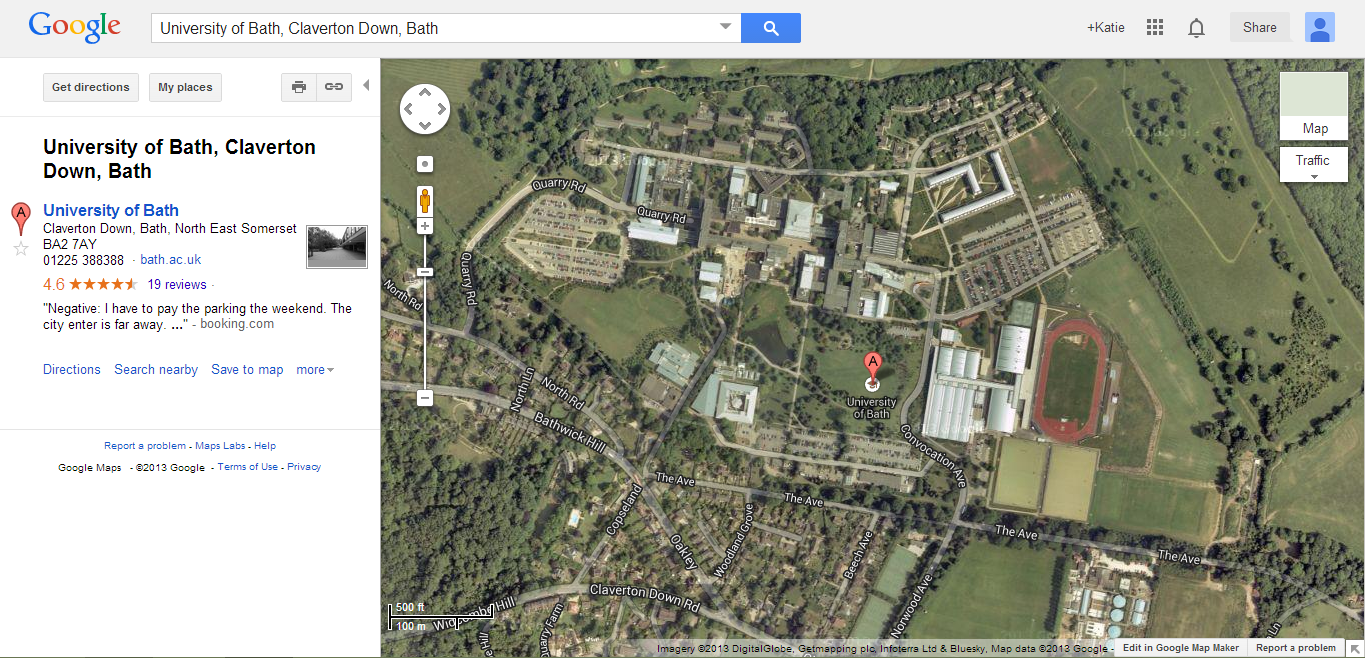
\includegraphics[keepaspectratio, width=\textwidth]{googlemapsexample.png}
\end{figure}

\subsection*{Second project we researched}
Placeholder for the domain research \#2.


%% \subsubsection*{Name of project we looked at 1}
%% Talk about the project a bit and the differences from our project.

%% \subsubsection*{Name of project we looked at 2}
%% Talk about the project a bit and the differences from our project.

%% \subsubsection*{Name of project we looked at 3}
%% Talk about the project a bit and the differences from our project.

\section*{Users \& significance to those users}
The tool we will be developing will be primarily aimed towards the students of Bath University.  The GPS navigation system will primarily be aimed at new students who do not know their way around the university. And the computer finder will primarily be aimed at students who are not living on campus as they will not be able to easily access a computer whilst on campus. Many of our key features are designed to aid the process of learning by reducing time wasted trying to find a suitable work station on campus. Our focus on the specific user group of students does not limit the use of our system, as the university has many industrial visitors who may not know their way around campus.

We have gathered the incentive to develop our system as all members of the team have been in the position of being lost on campus, and thought that the use of a route planner would be beneficial. In addition to this, as second year students now living off campus, we are finding it increasingly difficult to find computers to do work and would benefit from a system similar to the one we are proposing.  Although there is a web page that tells you if there are computers available, it does not inform you if the room currently in use and it is a laborious process to try and access the information relevant. We are striving to develop an application combines all the key aspects of systems, whilst being simple and easy to use so that the user only needs to use our application to find the relevant information.

\clearpage
\section*{Programme and Methodology}
\subsection*{Overall aims of the project}
After deciding on an idea for a project, the team laid out some goals which we would like to achieve, which are separate from the actual implementation. These should enable us to work effectively in a team, and to demonstrate our skills in software engineering. We can also use these goals at the end of the project to assess our performance, and analyse how well the project has gone.

At the highest level, we aim to create a working application which informs students of the location of free computers around campus, and uses GPS navigation to direct the student to the closest free computer. We aim to do this through the effective use of our design model, as well as user involvement through requirements gathering and also during testing.

Another aim is to improve on the existing systems available to students. We wish to create something that is both more usable and more functional than anything that exists in the same domain. To achieve this, we must first carry out research on the current systems, and interview potential users, to find out what areas we can improve in. More generally, we must find out more about usability and also what are the main components a system needs to make it more usable.
\subsection*{Other features of the application}
\begin{description}
\item[Free Computers] \hfill \\
This feature will provide the users with the real time information about free computers available on campus so that they don't have to look around  for computers. For this we needed real time information regarding the availability of computers at any current moment. After doing some research we found out that this information can be obtained from BUCS services website: http://www.bath.ac.uk/bucs/services/pacs/where.html
Our goal is to extract relevant information regarding free computers from this website, save the information in a data structure and apply algorithms to find the nearest computer room from user's current position.
\item[Weather widget] \hfill \\
This feature will provide the users with the real time information about the weather on campus. Lectures and Examinations are re-scheduled and sometimes cancelled due to bad weather conditions. Such a feature will be very helpful for the students since they can check the weather status directly from their smart phones. For this feature we need real time information regarding the weather at any current moment. Our goal is to  present this information using the Android weather widget. One additional feature we are adding to this is the background image of the application will change automatically depending on the weather conditions.
\item[Restaurant, Café, Shop finder] \hfill \\
This feature will provide the users with information regarding various shops and eateries on campus. A user can simply click an image representing food or a café and the application will guide the user to the nearest location.
\end{description}

\begin{figure}[H]
 \caption{Main menu prototype}
 \centering
 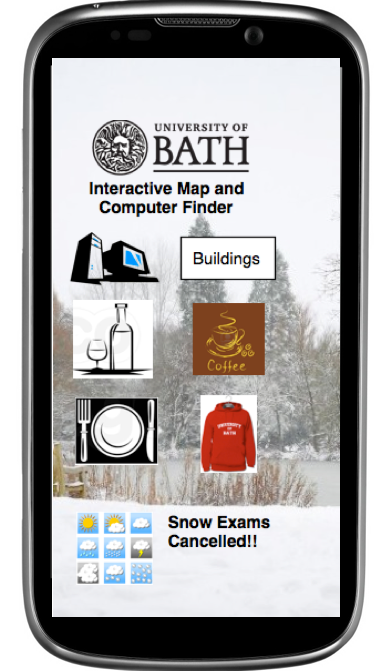
\includegraphics[keepaspectratio, scale=0.4]{prototype.png}
\end{figure}

\section*{System and programming platforms}
We're going to target Android based devices. The reasons are:
\begin{enumerate}
\item{Smartphones are becoming popularised among mobile users, and the largest proportion of them are using Android OS.}
\item{Android is open source. Which means it is easier of developers to customise software components and the software can be used on multiple devices.}
\item{Android app development is easier for developers who have experiences in Java programming.  And all of the team members have done java programming to some extent.}
\item{More software libraries are available to choose from.}
\item{Easier to test on Android phone.}
\end{enumerate}

Android in terms of the objectives of our system:
\begin{enumerate}
\item{Android provides a Map API that will make it easier to code and think about system elements such as buildings and shops as objects in the real world.}
\item{Android has a lot of documentation about how to design and manipulate graphical elements. This will make it easier to code the higher level graphical model.}
\item{Android provides a host of efficient data structures which are in-built and do not have to be coded from scratch. (Example: List View, List Adapter, Stacks, Trees etc.)}
\end{enumerate}

\begin{figure}[H]
 \caption{Android development environment}
 \centering
 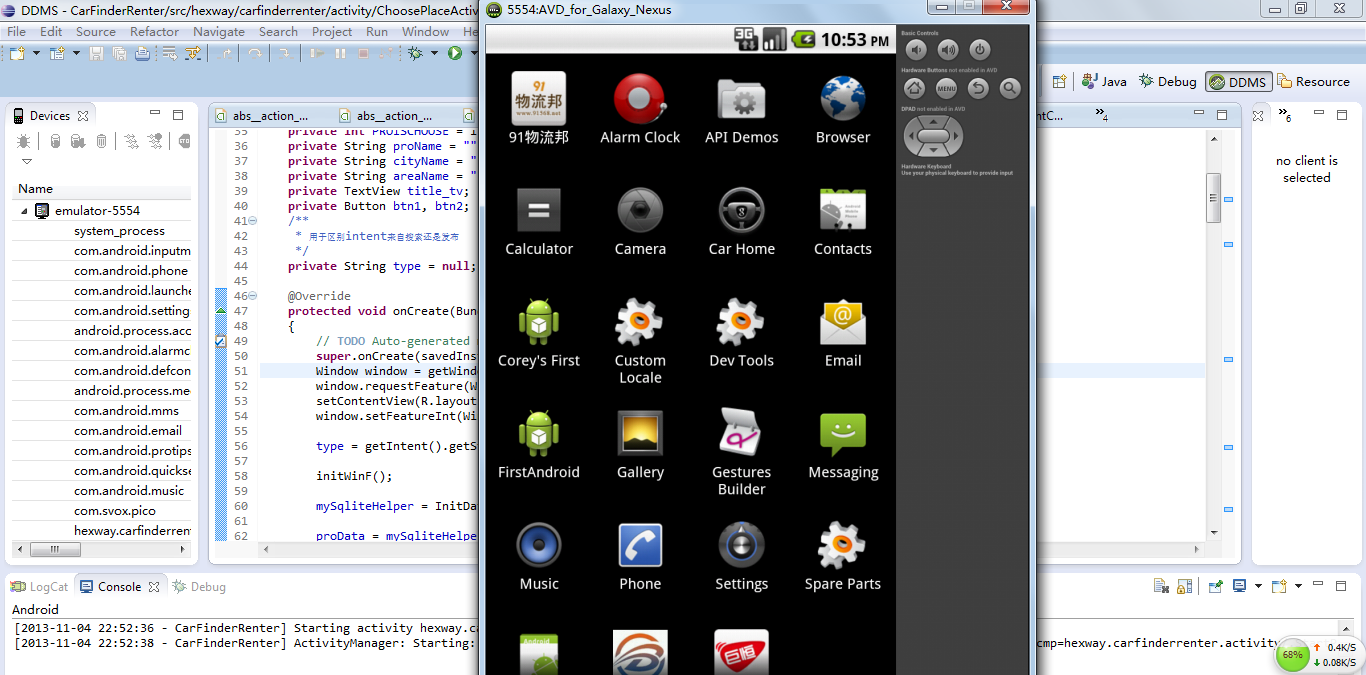
\includegraphics[keepaspectratio, width=\textwidth]{androiddev.png}
\end{figure}

\section*{Work plan}
During the project planning stage, each of our group members were delegated tasks and dealt with problems that came out during the development process.
This is how we approached our project planning:
\begin{enumerate}
\item{We created a Gantt chart allowing us to have an overview of the project process.}
\item{We created a GitHub version control repository to store the files and code for our project.}
\item{We formed a Facebook group that allows us to convey our opinions and ideas to the project instantly.}
\end{enumerate}
In order to keep track of the project, we did the following:
\begin{enumerate}
\item{Our group decided to meet at least once a week to discuss the progress we have made so far.}
\item{We recorded the start and end time of each of our group meetings and documented the entire meeting.}
\end{enumerate}

\begin{figure}[H]
 \caption{Meeting minutes}
 \centering
 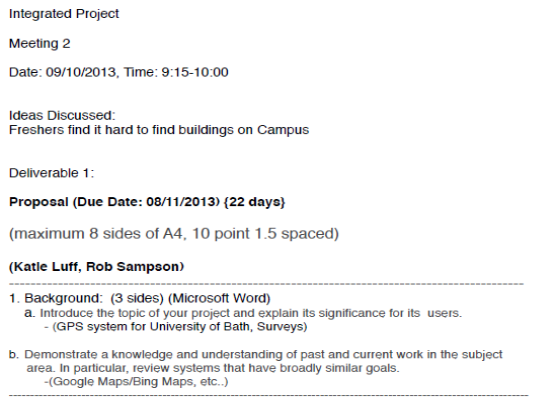
\includegraphics[keepaspectratio, scale=0.5]{meeting.png}
\end{figure}

\subsubsection*{Milestones for the project}
\begin{enumerate}
\item{Proposal stage}
\item{Design stage}
\item{Implementation stage}
\item{Test stage}
\item{Evaluation stage}
\end{enumerate}

% We put the generated chart on the last page.
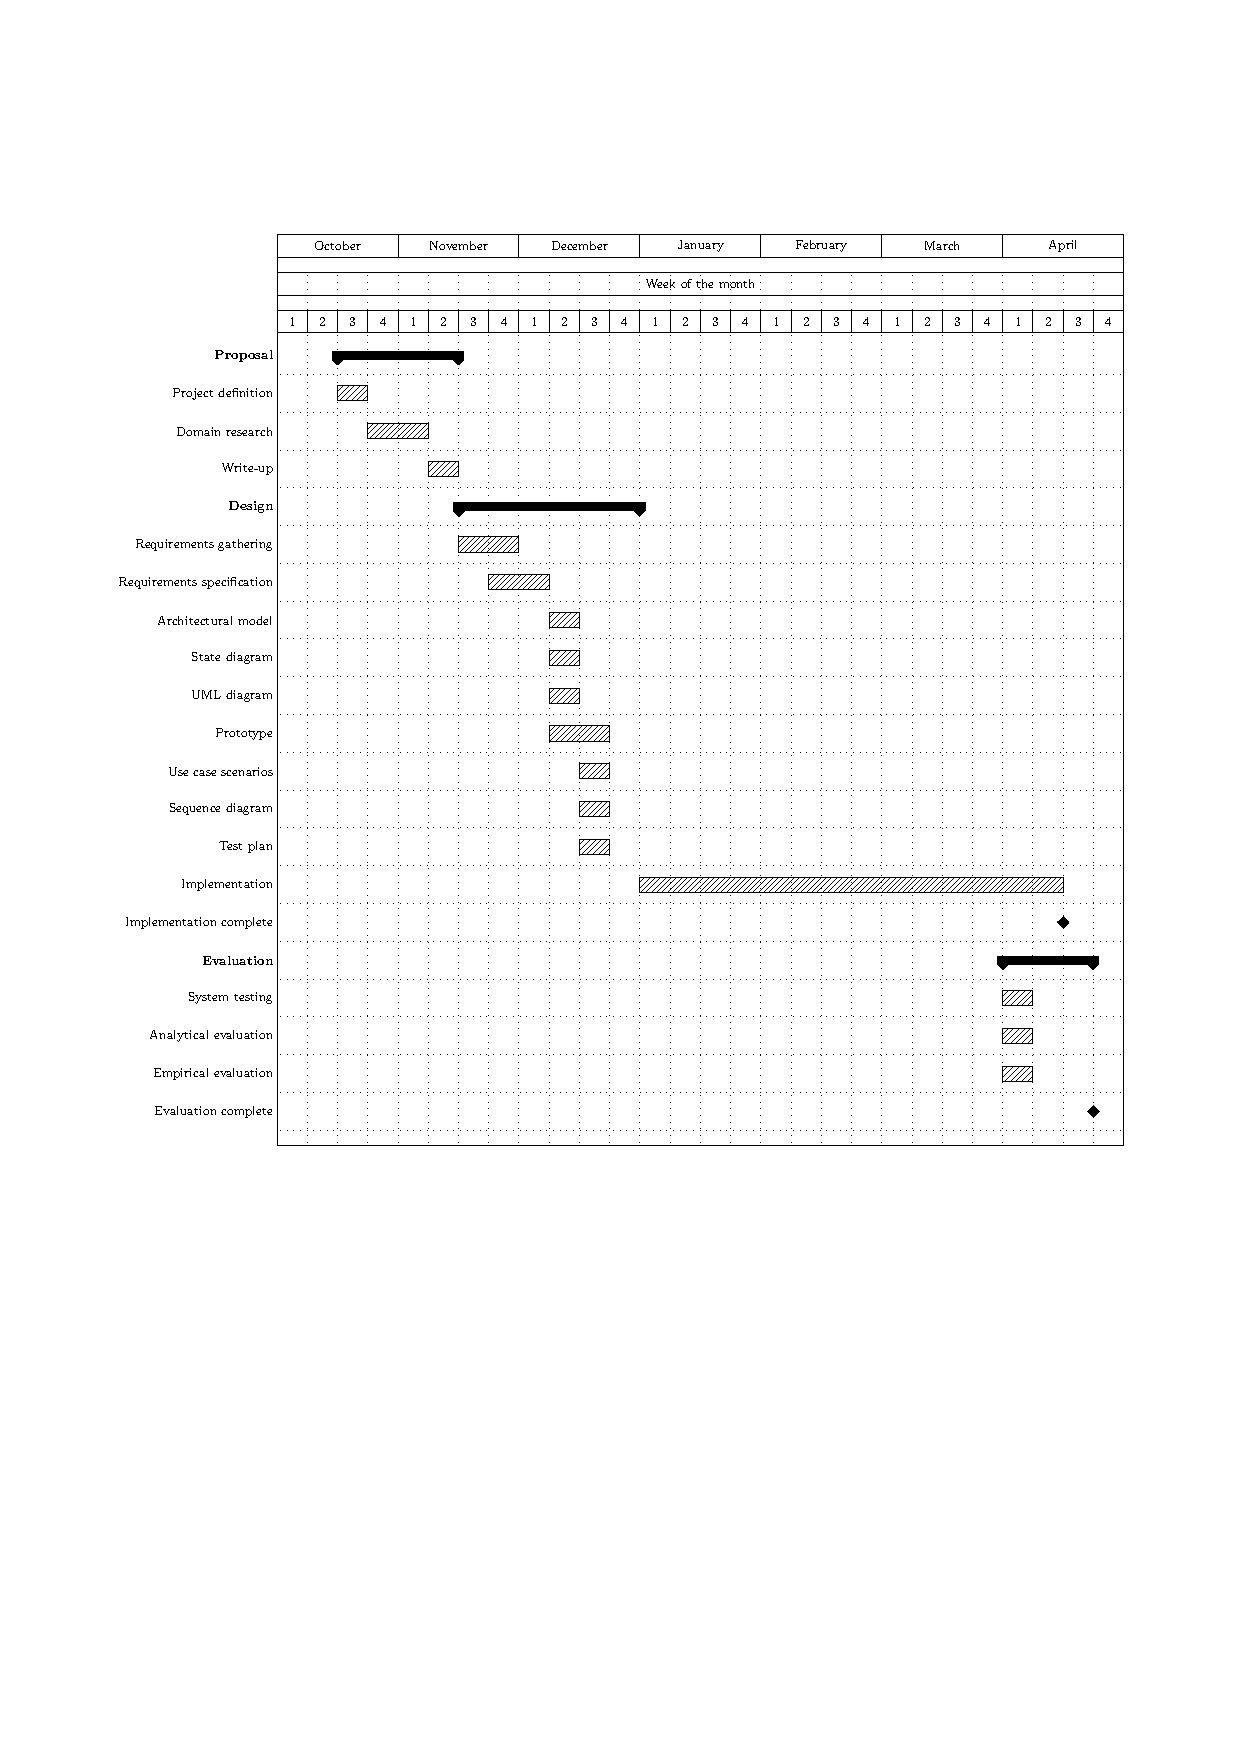
\includepdf[pages={1}]{ganttchart.pdf}

\end{document}
